\section{EXPERIMENTS}\label{sec:exp}
\begin{figure}[h]
    \centering
    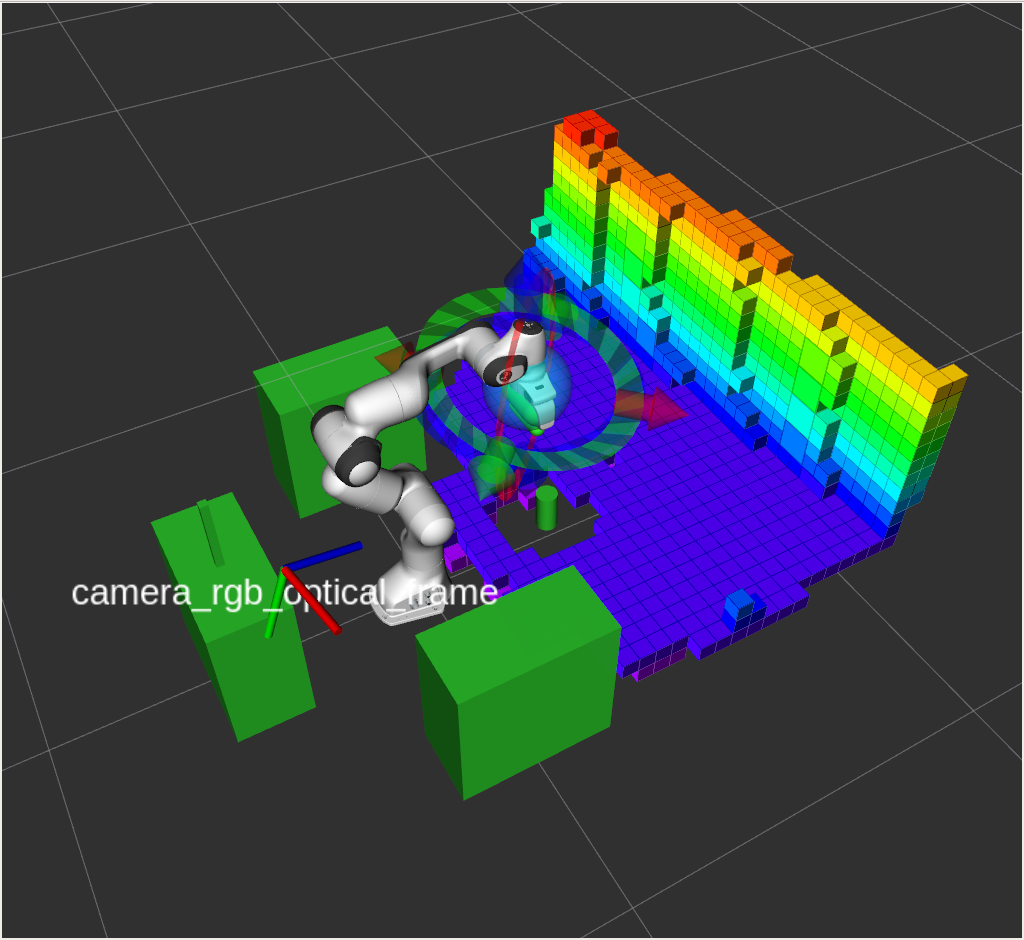
\includegraphics[width=5cm]{figures/exp2.png}
    \caption{Experimental setup}
    \label{fig:exp_setup}
\end{figure}
Due to the COVID-19 situation, we couldn't have the access to actual equipment and therefore proceed with simulations to experiment our algorithms for automatic pick-and-place grasping. 

Here we are using PANDA Robotic Arm with 7 degrees of freedom. We set the environment to contain one surface of wall and plane and three cubes of dimension 0.2$\times$0.4$\times$0.4 on the scene as shown in figure \ref{fig:exp_setup}, namely ``table1", ``table2" and ``table3".At the centre of each table, there is a bumper sensor to detect whether the table is occupied, namely ``bumper1", ``bumper2" and ``bumper3". A RGB-D camera is installed behind the robot, facing the wall, as shown in the \ref{fig:exp_setup}, for detecting objects on scene and forming point cloud. At the beginning, there is an object of dimension 0.02$\times$0.02$\times$0.2 on table2, which results in the bumper2 informing the robot that table2 is occupied, whereas the the other two bumper sensors inform the robot of the unoccupied surface. 

We will be having access to two information sources: the latest cylinder pose and the three bumper sensors' data. We used \texttt{PCL} and \texttt{ROS} in our simulation experiments. The cylinder pose is updated and published to the \textt{ROS} topic \texttt{/cylinder\_pose}, and the data from the bumper sensors is published to \textt{ROS} topic \texttt{/bumper1}, \texttt{/bumper2} and \texttt{/bumper3}, with \texttt{/bumper2} publishing boolean messages of ``true" and others publish ``false" to indicate only table2 is occupied at the beginning. 

Our experiments include testing the increase in extraction speed by applying various filters to the point cloud, the grasp of object, the process of pick-and-place to transfer the cylinder from the ground onto a free table, and the similar process of transferring the cylinder to an occupied table, which involves the removal of the object from the table. The results and discussions are detailed below.

\subsection{Increase in speed of cylinder extraction}
We have experimented various filters to speed up the cylinder extraction and test the time reduced. Below is the table to show the impact of the filtering on the time taken to extract the cylinder.
\begin{table}[h]
    \centering
    \begin{tabular}{|m{3cm}|m{1cm}|m{2cm}|}
        \hline
        Action & Number of points & Time of cylinder extraction (microseconds)  \\
         \hline
         RGB-D camera scan & 307200 & NA\\
         \hline
         Pass through filter to identify region of interest with range applied on z axis & 83484 & 4278 \\
         \hline
         Basic pass through filter + voxel grid filter to down sample the cloud & 5687 & 490\\
         \hline
         Basic pass through filter + pass through filter (fast filter) identifying the region of cylinder & 43122 & 2995\\
         \hline
         Basic pass through + voxel grid filter + fast filter & 2769 & 384\\
         \hline
    \end{tabular}
    \caption{Impact of applying different filters on speed of cylinder extraction}
    \label{tab:filters}
\end{table}

As shown in table \ref{tab:filters}, the voxel grid filter alone is more effective than fast filter alone in extraction speed boost. However, the combined effect of voxel grid and fast filter is the best.

\subsection{Grasp of cylinder from ground to surface}
\begin{figure}[h]
    \centering
    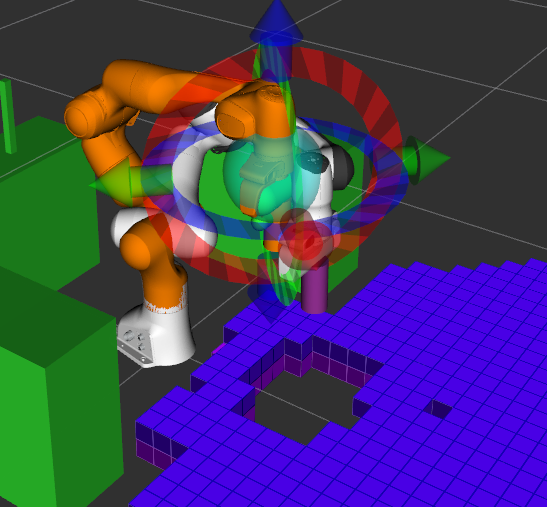
\includegraphics[width=4cm]{figures/grasp1.png}
    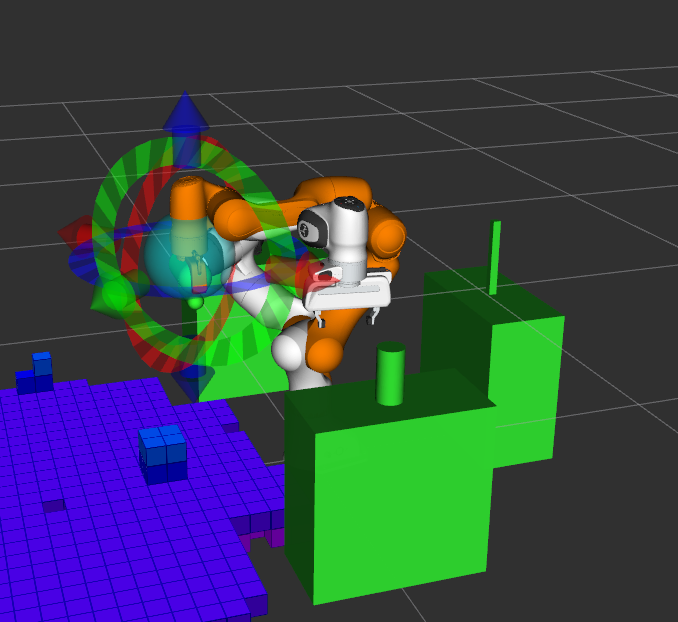
\includegraphics[width=4cm]{figures/grasp2.png}
    \caption{Picking up the cylinder and placing onto table1}
    \label{fig:grasp}
\end{figure}
As shown in figure \ref{fig:grasp}, upon receiving ``1" as the input, the robot successfully automatically locates the position of the cylinder, picks up the cylinder and place it onto table1.

\subsection{Automatic pick and place of cylinder in constrained environment}
\begin{figure}[h]
    \centering
    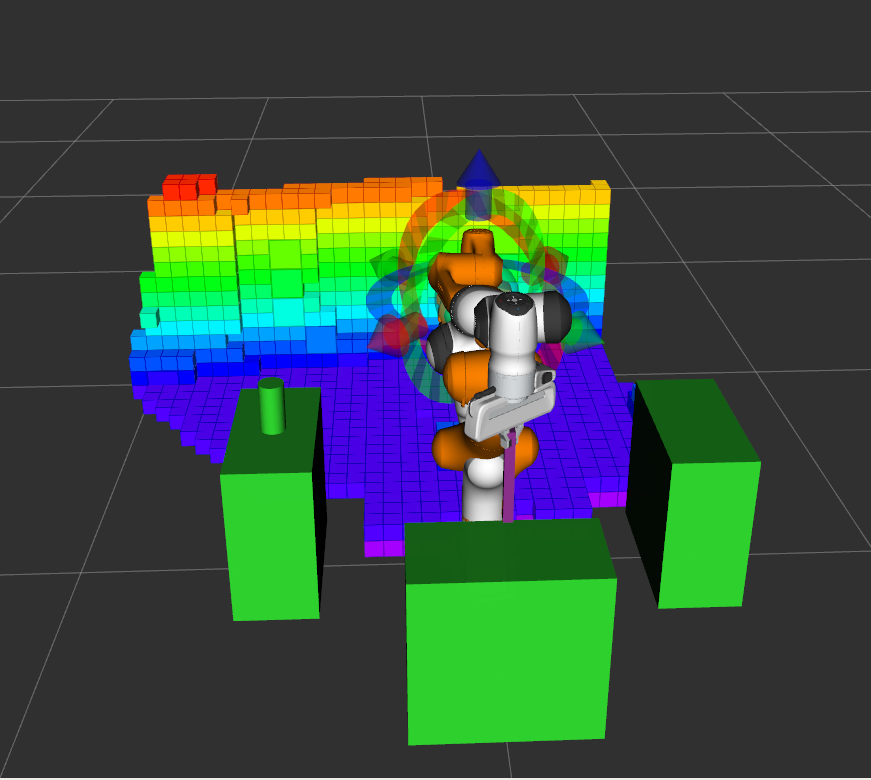
\includegraphics[width=4cm, height=4cm]{figures/2_pickStick.png}
    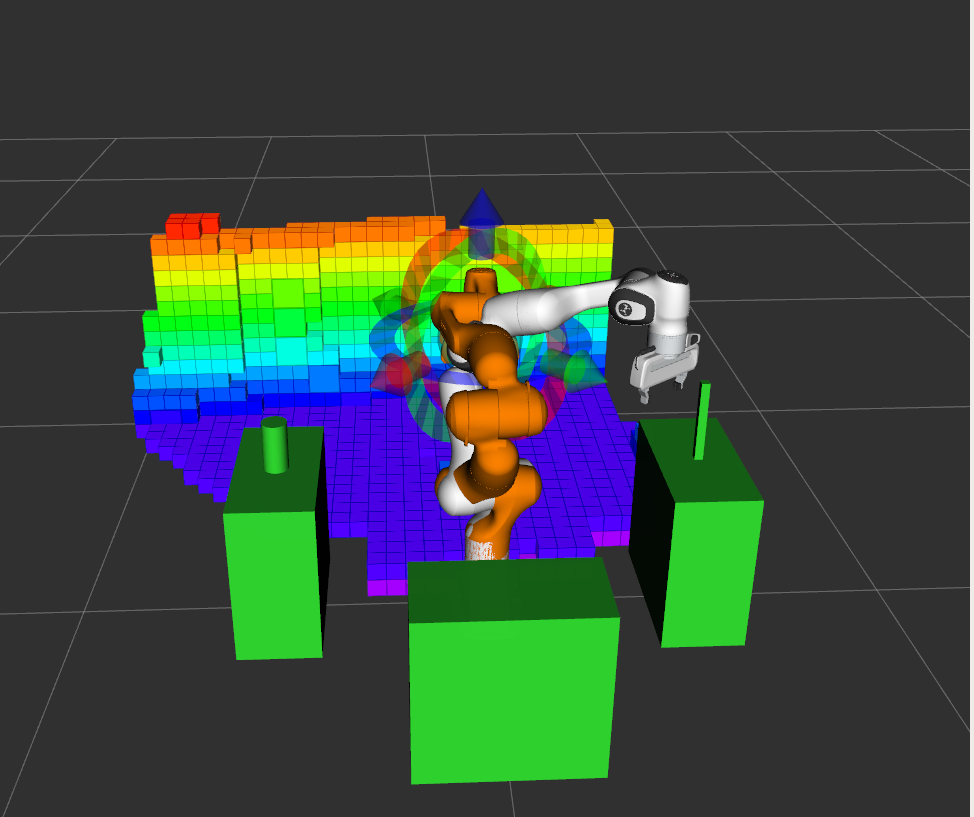
\includegraphics[width=4cm, height=4cm]{figures/2_placeStick.png}\\
    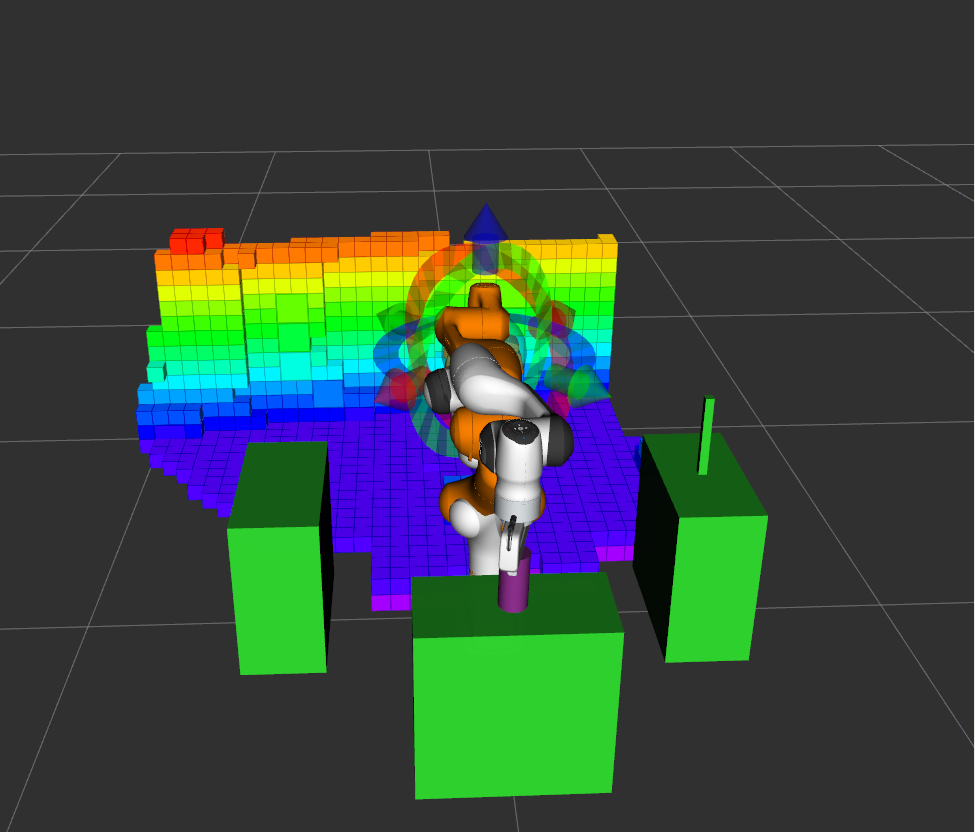
\includegraphics[width=4cm, height=4cm]{figures/2_pickCylinder.png}
    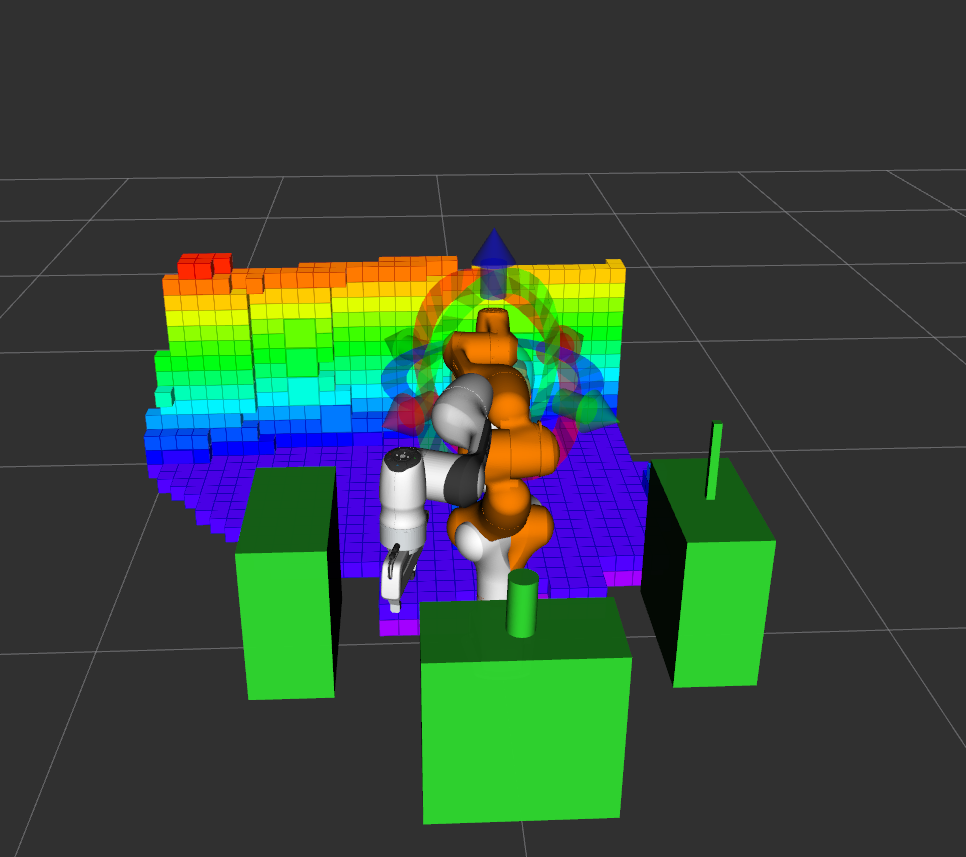
\includegraphics[width=4cm, height=4cm]{figures/2_placeCylinder.png}
    \caption{Picking up the cylinder and placing onto table1}
    \label{fig:2_pickPlace}
\end{figure}
As shown in the figure \ref{fig:2_pickPlace}, upon receiving instructions, the robot will automatically detect whether the designated table is occupied, and, if so, moves the occupant to another free table before placing the cylinder there. In this case, when the user input is ``2", the robot detects that there is an object on the table 2, and moves the object from table 2 to table 3 upon detecting that table 3 is empty, before moving the cylinder from table 1 to table 2. \\

From the simulated experiments, we can see that the algorithm we developed using RGB-D camera and bumper sensors can successfully detect the presence of objects on the surfaces and automate the process of pick-and-place of the target under the constraints of having obstructions on the surfaces. \\

However, the experiments conducted in the simulation are largely simplified. The context of the constraints in the environment can be much more complicated. For example, most objects may not be placed right at the center on the surface in real life, and therefore may not be detected if there is only one bumper sensor at the center of the table. It could also be that there are many obstructions on the scene and the RGB-D camera cannot detect the target of interest, therefore cannot generate the 3D point cloud of the object. These limitations need further considerations when conducting experiments in real life.